\subsection{Fantasia3D}\label{fantasia3D}

The model proposed by \citeauthor{chen2023fantasia3d} takes a different approach to generating 3D models from text input, in particular by disentangling geometry and appearance in the generated 3D models.
This method offers a more detailed rendering quality compared to conventional Neural Radiance Fields (NeRFs), which use volume rendering to combine the learning of surface geometry with pixel colors. This conventoional approach limits effective surface recovery, lacking the capability to track the surface of an object and tune detailed material and texture. In contrast, Fantasia3D achieves more realistic outputs with its hybrid scene representation of DMTet, ``which maintains a deformable tetrahedral grid and a differentiable mesh extraction layer; deformation can thus be learned through the layer to explicitly control the shape generation'' \citep{chen2023fantasia3d}

\begin{figure}[ht]
  \centering
    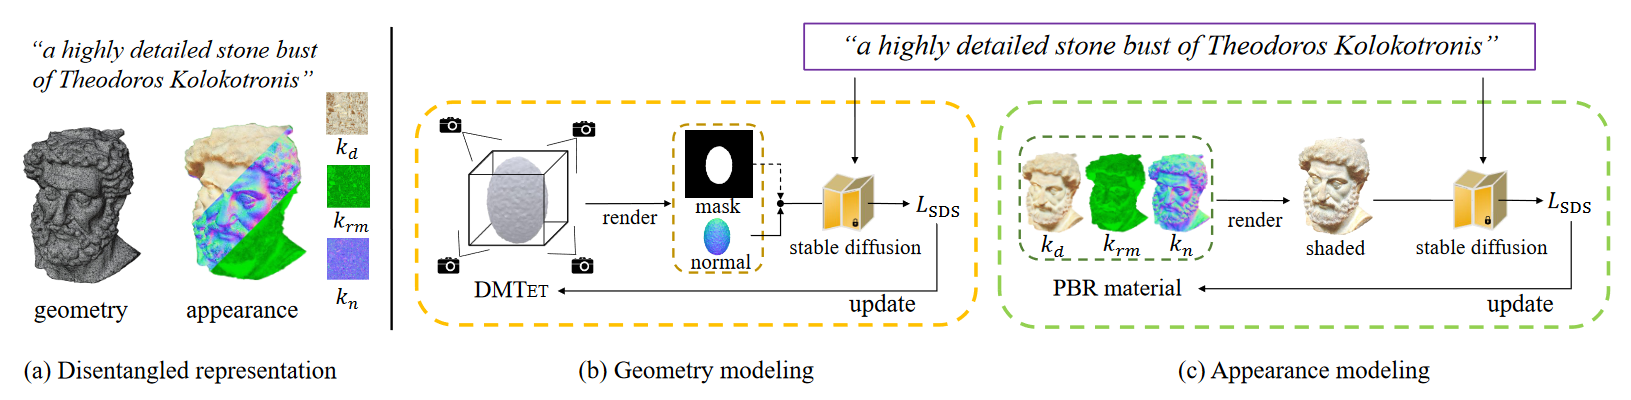
\includegraphics[width=1\columnwidth]{figures/Fantasia3D.png}
    \caption{Overview of Fantasia3D's workflow, disentangling geometry from appearance modeling and iteratively enhancing the quality using a refinment process \citep{chen2023fantasia3d}.}\label{fig:figureFantasia}
\end{figure}

In the geometry stage, Fantasia3D relies on a Deformable Mesh Tetrahedralization (DMTet), which parametrizes the 3D geometry as a Multi-Layer Perceptron (MLP) \(\Psi\). Initially, Fantasia3D renders and encodes surface normals and object masks extracted from DMTet. However, in later stages, the model refines its approach by using only the rendered normal map for shape encoding \citep{chen2023fantasia3d}. The default initialization of DMTet is an ellipsoid, but the model also accepts custom inputs.

Appearance Modeling involves training another MLP \( \Gamma \), which is responsible for applying the Bidirectional Reflectance Distribution Function (BRDF) \citep{chen2023fantasia3d} to a pre-learned DMTet. This function is crucial for ``predict[ing] parameters of surface material and supports high-quality 3D generation via photorealistic rendering'' \citep{chen2023fantasia3d}. The BRDF focuses on the diffuse parameter \(k_d\), the combined roughness and metallic parameter \(k_{rm}\), and the normal variation parameter \(k_n\) to achieve accurate shading of the geometry. These are predicted using the formula \((k_d, k_{rm}, k_n) = \Gamma(\beta(p); \gamma)\) by \citeauthor{chen2023fantasia3d}, where \(\beta(p)\) represents the surface properties at point \(p\) and \(\gamma\) denotes network parameters.

Both MLPs (\(\Gamma\) for appearance and \(\Psi\) for geometry) undergo a refinement process, using a pre-trained Stable Diffusion model \citep{rombachStableDiffusion}. This model improves the capabilities of \(\Gamma\) and \(\Psi\), ensuring that they accurately interpret and render 3D shapes and textures. A key aspect of this refinement is the use of Score Distillation Sampling (SDS) loss \citep{mildenhallNERF} for optimization. In this process, SDS loss functions by comparing the true image with the one generated by Fantasia3D. This comparison is achieved through ray casting, where rays are projected for each pixel in the scene. The model then renders the color of each ray, effectively translating the 3D model into a 2D image. This step allows the model to evaluate and adjust its rendering based on how accurately it replicates the true image of Stable Diffusion. By iterating this process vor multiple viewpoints, the model continually improves its accuracy in rendering photorealistic images, ensuring that the final output is as close to the actual image as possible.

Fantasia3D offers a high degree of user interactivity, permitting the incorporation of both custom and predefined generic 3D shapes, thus greatly enhancing the versatility and user engagement in the content creation process. The separation of geometry and appearance generation also ensures compatibility with widely-used graphics engines \citep{chen2023fantasia3d}. Despite its capabilities in creating high-quality 3D models from textual descriptions, Fantasia3D encounters specific challenges. One notable limitation is its struggle with accurately generating complex geometries like hair, fur, and grass \citep{chen2023fantasia3d}. Furthermore, the model is currently not able to generate complete scenes as focus is currently lying on individual object generation \citep{chen2023fantasia3d}.